%!TEX root = main.tex

\chapter{Estado del arte}
\section{Particle Swarm Optimization}
Como se introduce en el artículo de Kaveh \cite{Psoexplain14}, el algoritmo \emph{Particle Swarm Optimization} es una metaheurística inspirada en el comportamiento social de poblaciones de enjambres. Este simula la conducta colectiva a través de partículas (soluciones) que se mueven dentro de un espacio de búsqueda mediante factores individuales y colectivos, que direccionan el movimiento a zonas de ``buena calidad'', determinadas por una función objetivo (\emph{fitness function}).\\
Se dice enjambre a un conjunto de partículas en un espacio de búsqueda, cuya posición $x$ representa el vector solución, el cual varía dentro de dicho espacio a velocidad $v$. El modelo clásico presentado por Kennedy y Eberhart\cite{Kennedy95}, describe la variación de la velocidad y de la posición de las partículas como se presenta a continuación:
\begin{align*}
    v_{i,j}^{k+1} = v_{i,j}^{k} + c_{1}r_{1}(xbest_{i,j}^k - x_{i,j}^k) + c_{2}r_{2}(xgbest_{j}^{k} - x_{i,j}^k)\\
    x_{i,j}^{k+1} = x_{i,j}^{k} + v_{i,j}^{k+1}
\end{align*}    
Como se explica en Kaveh \cite{Psoexplain14} $x_{i,j}^{k}$ y $v_{i,j}^{k}$ son la $j$-ésima componente de la posición y la velocidad de la partícula $i$ respectivamente en la iteración o tiempo $k$, $r_{1}$ y $r_{2}$ son número aleatorios uniformes que varían de 0 a 1, $xbest_i$ y $xgbest$ representan las mejores soluciones alcanzadas por la partícula y por el enjambre respectivamente, $c_1$ y $c_2$ son parámetros que representan la confianza en la solución indiviual de la partícula (parámetro cognitivo) y la incidencia del aspecto colectivo o solución global (parámetro social), respectivamente. Un esquema de la interacción de estos componentes se aprecia en la figura \ref{fig:move_part}\\
\begin{figure}[h!]
    \centering    
    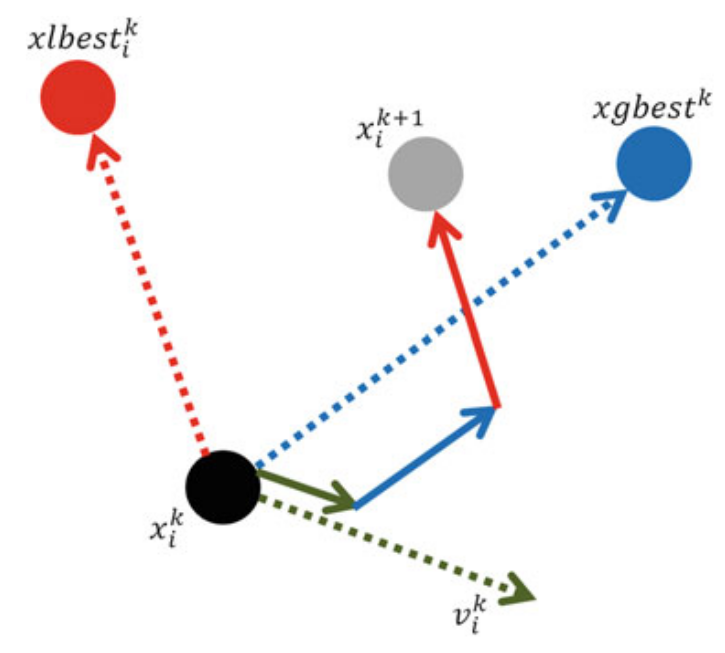
\includegraphics[height=50mm]{figures/move_particle.png} 
    \caption{Movimiento de una partícula}
    \label{fig:move_part}
\end{figure}
A modo de equilibrar la incidencia de la velocidad previa de la partícula, se añade un factor que escala esta velocidad, dado que como se explica en Kaveh \cite{Psoexplain14}, si la velocidad previa se elimina, las partículas quedan atrapadas en una región local, pero si se le da demasiado peso, converge rápidamente a un óptimo conocido. Por esto, la forma del PSO base actual, tiene un parámetro $w$, que representa la incidencia de la velocidad previa (factor de inercia), por lo que ahora tenemos que la partícula se mueve acorde a: 
\begin{align*}
    v_{i,j}^{k+1} = wv_{i,j}^{k} + c_{1}r_{1}(xbest_{i,j}^k - x_{i,j}^k) + c_{2}r_{2}(xgbest_{j}^{k} - x_{i,j}^k)\\
\end{align*}    
En el trabajo inicialmente citado, se puede ver una revisión completa del estado del arte del método \emph{Particle Swarm Optimization}, mostrando las distintas modificaciones y alternativas propuestas por la literatura que pretenden mejorar aspectos como la configuración de los parámetros (inercia, cognitivo, social, aleatorios), los problemas asociados a la convergencia prematura, topologías o estructuras del enjambre que modifican la comunicación entre partículas (o la incidencia de las soluciones globales y particulares), sesgos en la búsqueda por la forma de la región o por la interacción de las partículas (operadores de combinación como el promedio, que tienden a centrar la búsqueda en determinada región), algoritmos híbridos con PSO y la versión discreta de este método. 
\section{Velocidad del viento}
\section{Dirección del viento}
